\chapter{設計}
\label{chap:design}

本章では、本研究において提案する、マイコン向けWebAssembly実行環境の設計を示す。

\section{全体の構成}

本研究で提案する実行環境は、インターネット上から取得したWebAssemblyプログラムをマイコン上で実行するために、HTTP通信のためのクライアントとWebAssemblyプログラムの実行エンジンから構成される。

なお、WebAssemblyは複数モジュールにおける動的リンクの手段も規定しているため、モジュールを分割してマイコン側でリンクする事でキャッシュ効率を高められると考えられるが、マイコンという実行環境の制約上プログラム全体のサイズは限定されると考え、本研究では単一のモジュールのみを取得し実行するユースケースを想定した。

図\ref{fig:wasm_design}に、本実行環境におけるWebAssemblyプログラムの実行フローを示す。

\section{WebAssemblyプログラムの取得と実行}

マイコンの初回起動後、WebAssembly実行エンジンはHTTPクライアントに実行するためのプログラムを要求する。
HTTPクライアントはファームウェア書き込み時に指定したURLを用いて、HTTPサーバからWebAssemblyバイナリを取得し、実行エンジンへ渡す。
実行エンジンは受け取ったWebAssemblyバイナリをパースし、エントリーポイントから実行する。
WebAssemblyプログラムが実行を終える、または明示的に実行エンジン側へ通知を行うと、実行エンジンは現在のWebAssemblyバイナリを破棄し、次に実行するためのWebAssemblyバイナリを再度HTTPクライアントへ要求する。

\begin{figure}[htbp]
  \caption{本実行環境におけるWebAssemblyプログラム実行フロー}
  \label{fig:wasm_design}
  \begin{center}
    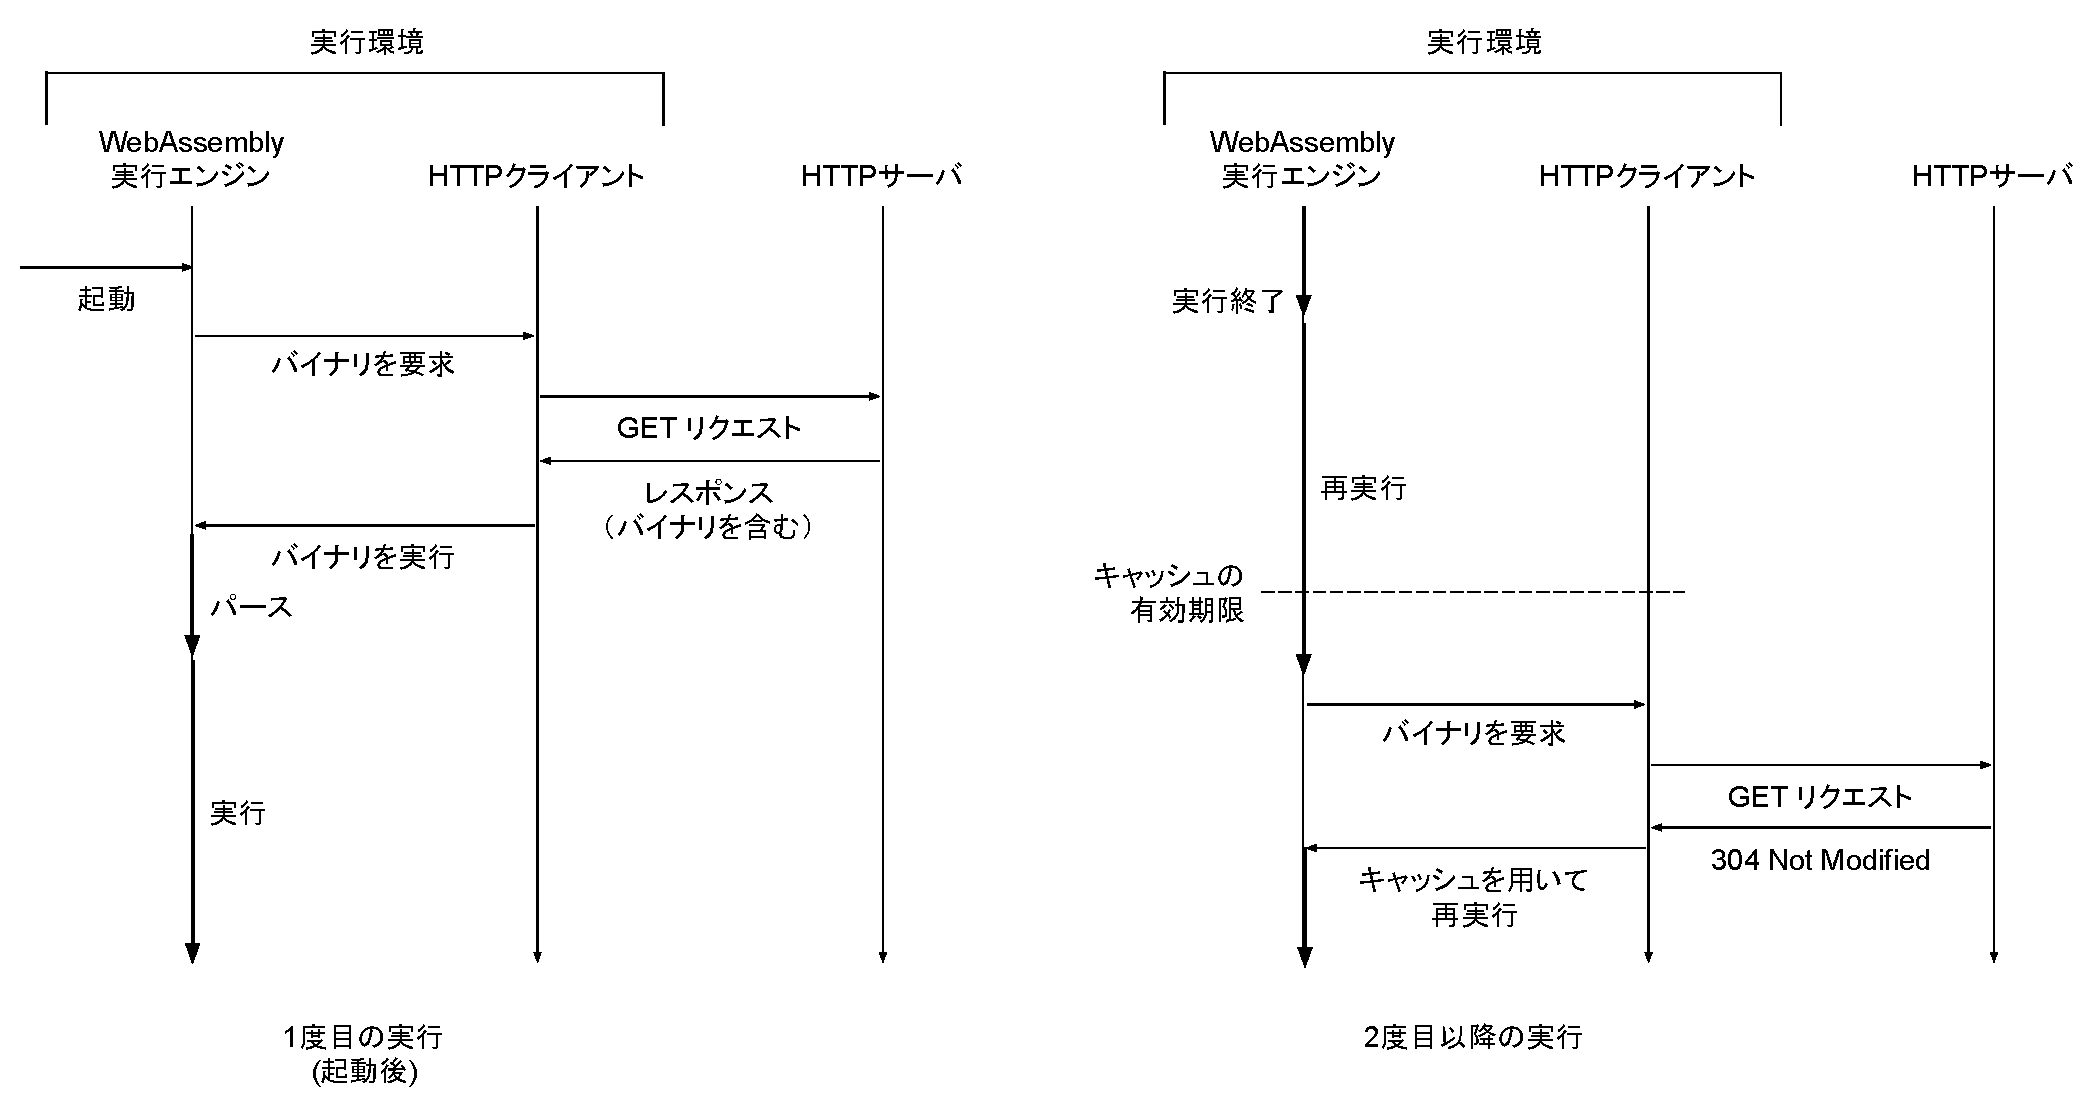
\includegraphics[bb=0 0 1000 530,width=15cm]{img/wasm_design.pdf}
  \end{center}
\end{figure}

\section{WebAssemblyバイナリ取得の制御}

本実行環境のHTTPクライアントは標準的なHTTPユーザーエージェントとして振舞うことで、特殊なサーバ実装を用意することなく、HTTPレスポンスによりWebAssemblyバイナリ取得の制御を行うことができる。

HTTPサーバからのレスポンスヘッダがキャッシュを許可していれば、キャッシュが有効な間、実行環境はWebAssemblyバイナリを再取得せずに実行し続ける事ができる。
また、実行環境はレスポンスに含まれる{\tt ETag}や{\tt Last-Modified}といった値を保持し、WebAssemblyバイナリ再取得時のリクエストに含めることで、バイナリに変更がない場合はレスポンスを{\tt 304 Not Modified}ステータスコードのみにできる。
適切にキャッシュを利用することで、通信のための計算負荷、通信帯域を節約できるだけでなく、WebAssemblyモジュールのパースや初期化を再度行うことなく処理を再開できる。

WebAssemblyバイナリの取得元URLは、バイナリ取得時のHTTPレスポンスステータスコードとして{\tt 301 Moved Permanently}を設定することにより恒久的に、また{\tt 302 Found}や{\tt 307 Temporary Redirect}を設定することにより一時的に、変更することができる。

また、必要に応じて、Web通信で標準的に用いられる認証や圧縮といった技術を用いて、通信の安全性や効率を高めることができる。
